%   ------------------------------------------------------------------------
\FloatBarrier
\subsection{Geração do sprite em back view}
\label{s.gemini.backview}

Para a geração do sprite em back view, foi usado como referência o sprite em front view (Figura \ref{fig:geminiProPablo}) e o sprite em side view (Figura \ref{fig:geminiProSideEdicaoMelhorAposEdicao}). Inicialmente, o modelo interpretou errado a instrução de fazer o personagem virado para o norte, gerando o sprite em front view com deformações de pixels no rosto, que aparentavam formar um sorriso. Isso pode ser visto na Figura \ref{fig:GeminiProSpriteSegundoRosto}.

\begin{figure}[htbp]
    \centering
    \caption{\small Sprite gerado em back view com pixels errados no rosto no Gemini Pro}
    \label{fig:GeminiProSpriteSegundoRosto}
    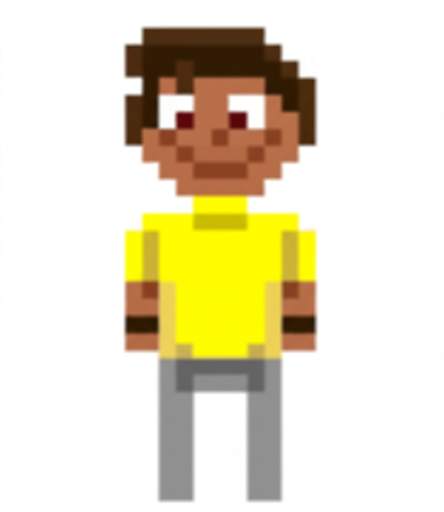
\includegraphics[width=0.3\linewidth]{figs/geminiPro/chat12/01_res2.png}
    \legend{\small Fonte: Elaborada pela autora, utilizando a ferramenta Gemini Pro.}
\end{figure}

Na interação seguinte, foi especificado melhor que o personagem deveria estar de costas. Os resultados gerados foram todos satisfatórios, mantendo alta consistência com o estilo e o personagem, como pode ser visto na Figura \ref{fig:GeminiProBackMelhor}. A olho nu, os sprites parecem manter o padrão pixel perfect, sendo facilmente exportados para aplicativos de edição de pixel art.

\begin{figure}[htbp]
    \centering
    \caption{\small Melhor sprite gerado em back view no Gemini Pro}
    \label{fig:GeminiProBackMelhor}
    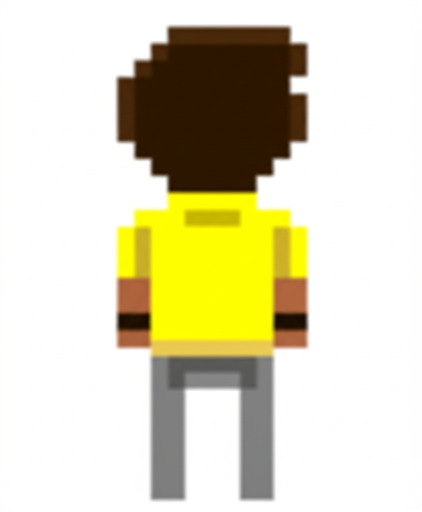
\includegraphics[width=0.3\linewidth]{figs/geminiPro/chat12/02_res2.png}
    \legend{\small Fonte: Elaborada pela autora, utilizando a ferramenta Gemini Pro.}
\end{figure}

Apesar disso, foi notado que os tons de cores não eram exatamente idênticos aos do sprite original, sendo necessário que a imagem passasse por essa correção. Assim como foi feito com o sprite em side view, a imagem foi exportada para o Pixilart, como pode ser visto na Figura \ref{fig:geminiProBackEdicaoMelhor}. Após isso, a imagem foi colocada na ferramenta Pixel Lab, onde foi realizado o pós-processamento (detalhado na Seção \ref{s.pixelLab}).

\begin{figure}[htbp]
    \centering
    \caption{\small Processo de edição do melhor sprite em back view no Pixirart}
    \label{fig:geminiProBackEdicaoMelhor}
    \begin{subfigure}{0.45\linewidth}
        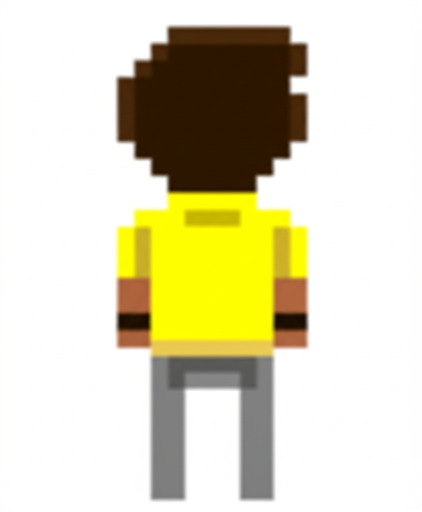
\includegraphics[width=1\linewidth]{figs/geminiPro/chat12/02_res2.png}
        \caption{\small Melhor sprite em back view gerado pelo Gemini Pro antes de converter para pixel perfect}
        \label{fig:geminiProBackEdicaoMelhorAntesEdicao}
    \end{subfigure}\hfill
    \begin{subfigure}{0.45\linewidth}
        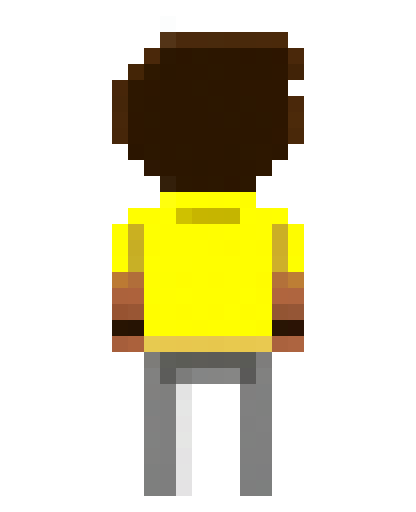
\includegraphics[width=1\linewidth]{figs/geminiPro/back_pixel_grande.png}
        \caption{\small Sprite em back view após conversão para pixels no Pixilart}
        \label{fig:geminiProBackEdicaoMelhorAposConversao}
    \end{subfigure}\hfill
    \legend{\small Fonte: Elaborada pela autora.}
\end{figure}

Os resultados dos testes descritos nesta seção podem ser consultados nas Figuras \ref{fig:geminiProBack1} e \ref{fig:geminiProBack2}.

Em geral, os testes para a geração do sprite em back view revelaram uma capacidade de consistência ainda maior do que a observada anteriormente. O modelo foi capaz de simular o padrão pixel perfect com alta fidelidade a olho nu, um feito impressionante para um modelo de IA generativo que não é especializado nesse estilo, solidificando ainda mais o Gemini Pro como a ferramenta mais eficiente para a criação de poses base para animações 2D.

